%!TEX root = Report.tex


\chapter{Displacement Historgram}


\begin{figure}[H]
\centering
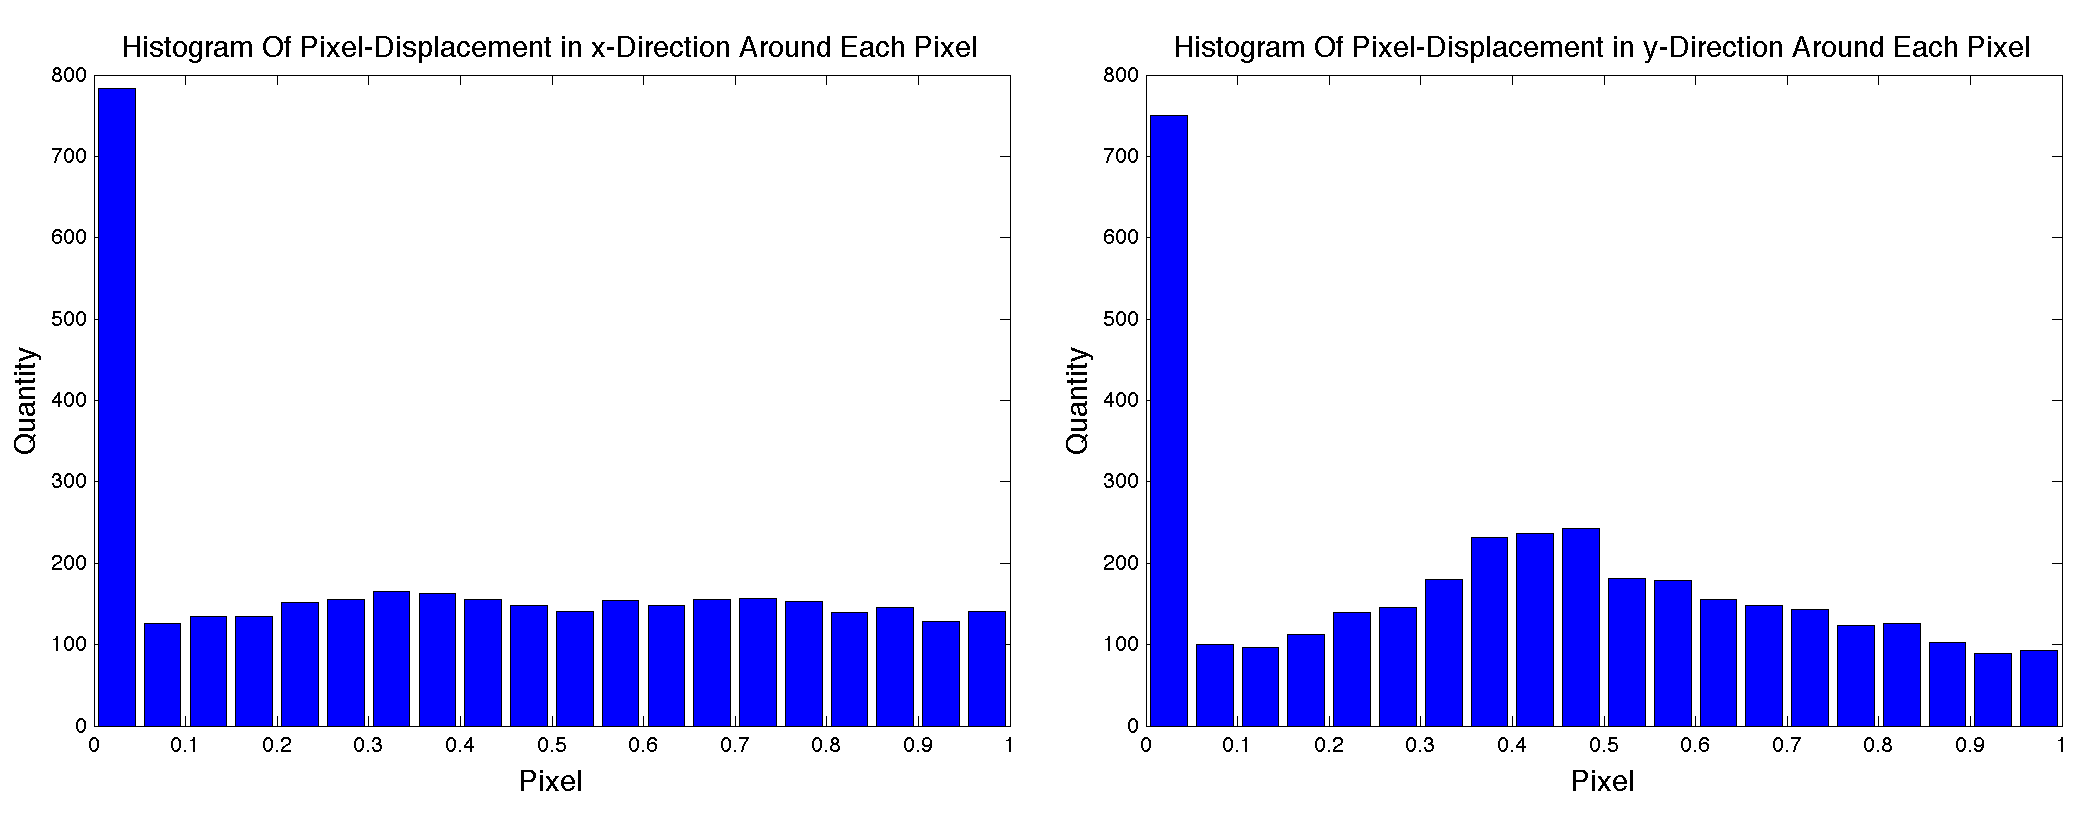
\includegraphics[width=0.9\textwidth]{pics/figure6_run3.png}
\caption{Histograms Of Displacements in $x$ and $y$ Directions For The Third Run}
\label{pic:6r3}
\end{figure}


\chapter{Correlation Composite Images}
\begin{figure}[h]
\centering
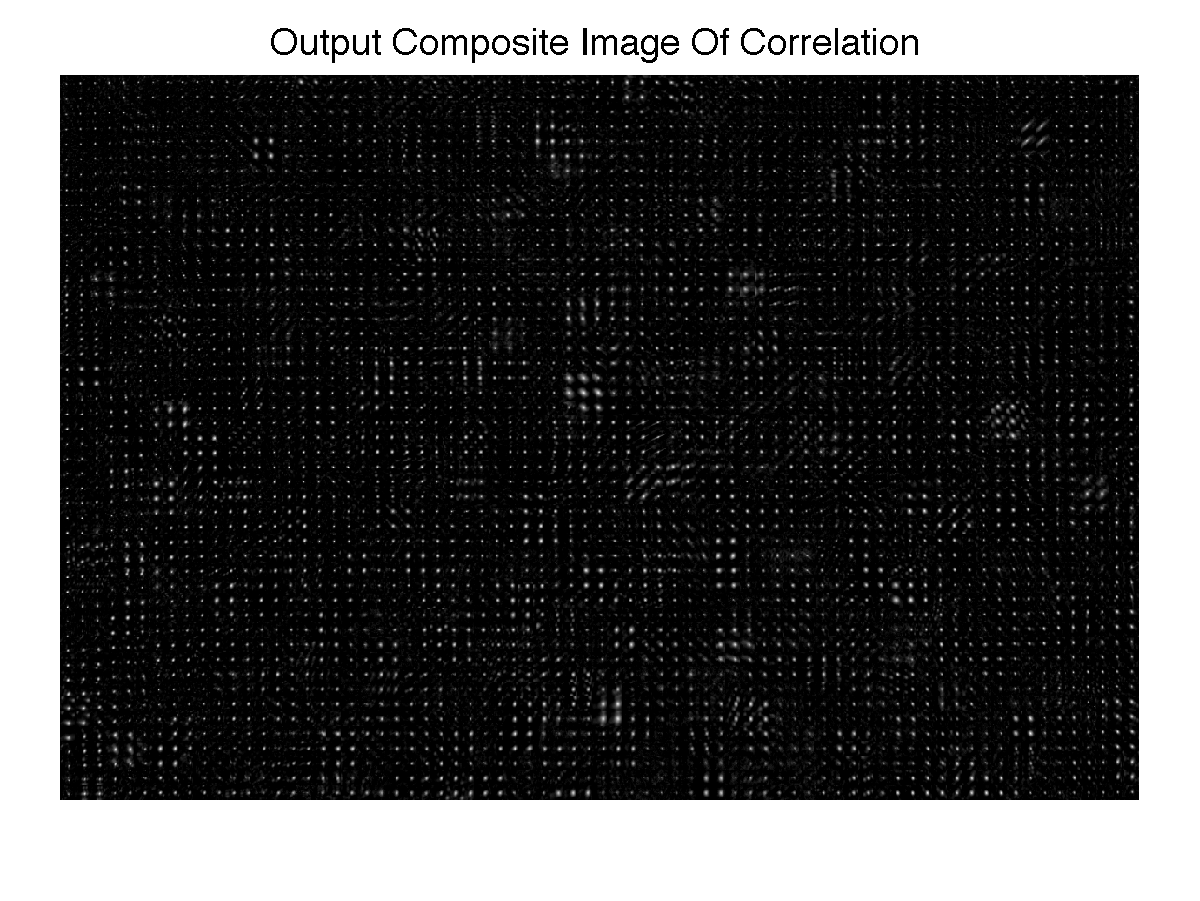
\includegraphics[width=\textwidth]{pics/figure1_run2.png}
\caption{Composite Compound Image For Third Run}
\label{pic:1r2}
\end{figure}


\begin{figure}[h]
\centering
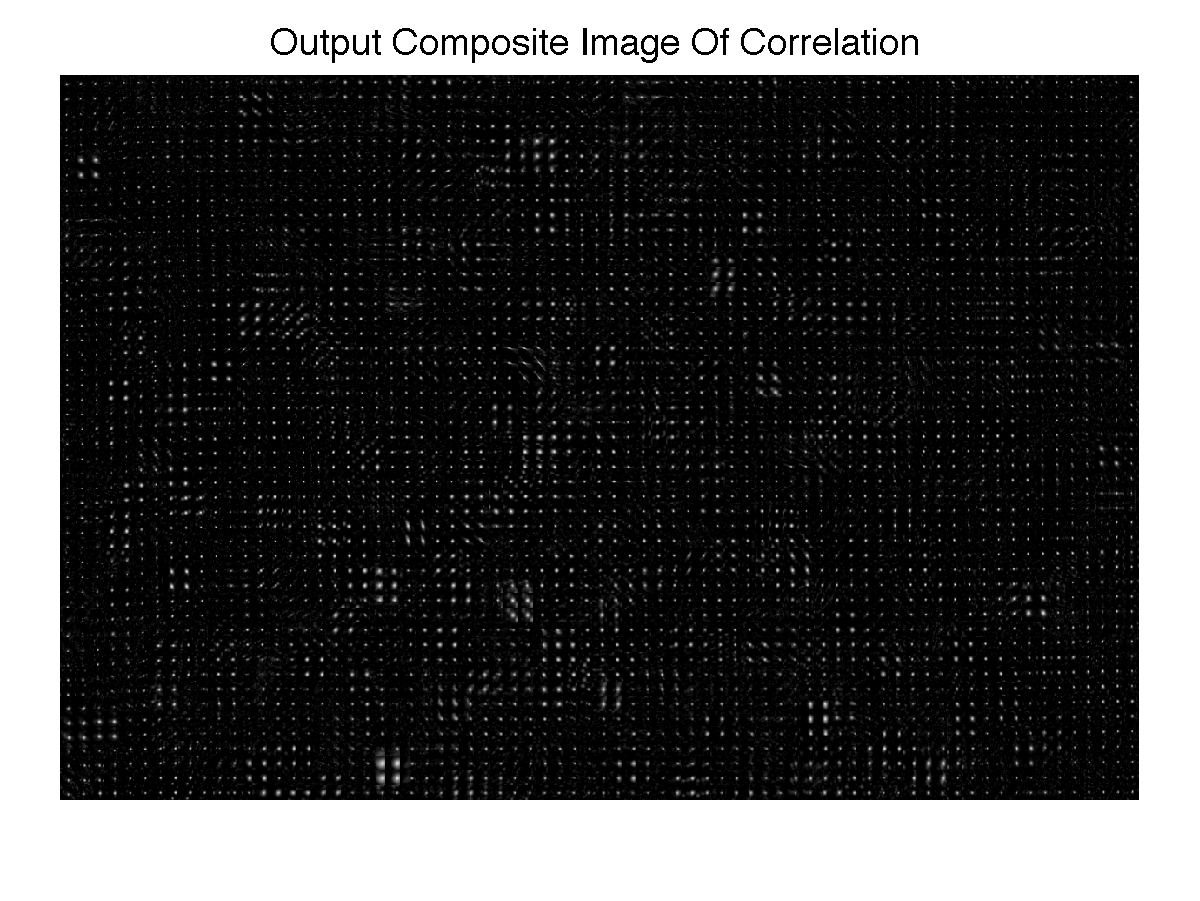
\includegraphics[width=\textwidth]{pics/figure1_run3.png}
\caption{Composite Compound Image For Third Run}
\label{pic:1r3}
\end{figure}




\fancypagestyle{lscapedplain}{%
  \fancyhf{}
  \fancyfoot{%
    \tikz[remember picture,overlay]
      \node[outer sep=1cm,above,rotate=90] at (current page.east) {\thepage};}
}

\chapter{MATLAB Code}\label{c:datasheets}




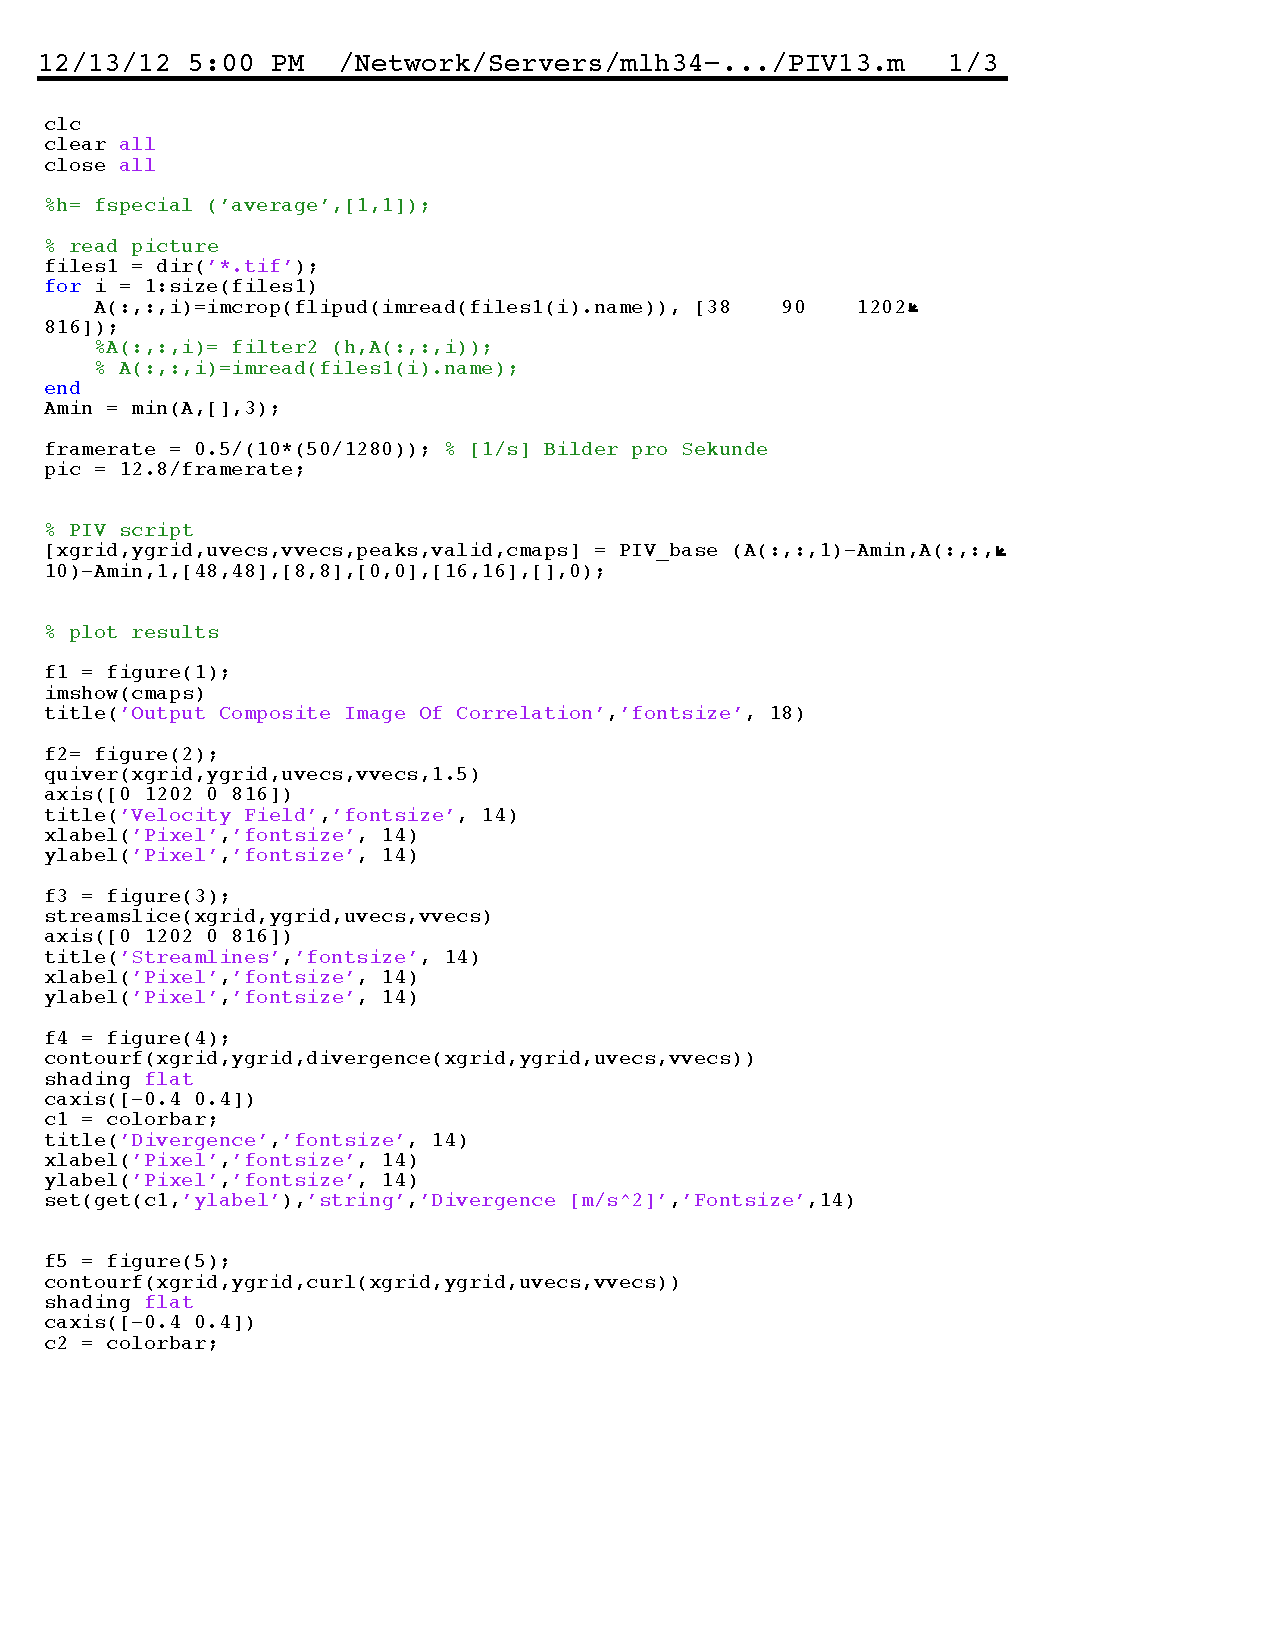
\includepdf[pages=-,frame=true, scale=0.9]{pics/code.pdf}

%\includepdf[pages={1,3,4-5},angle=0,nup=2x2,frame=true, scale=0.9]{datasheets/PicDatasheet.pdf}
%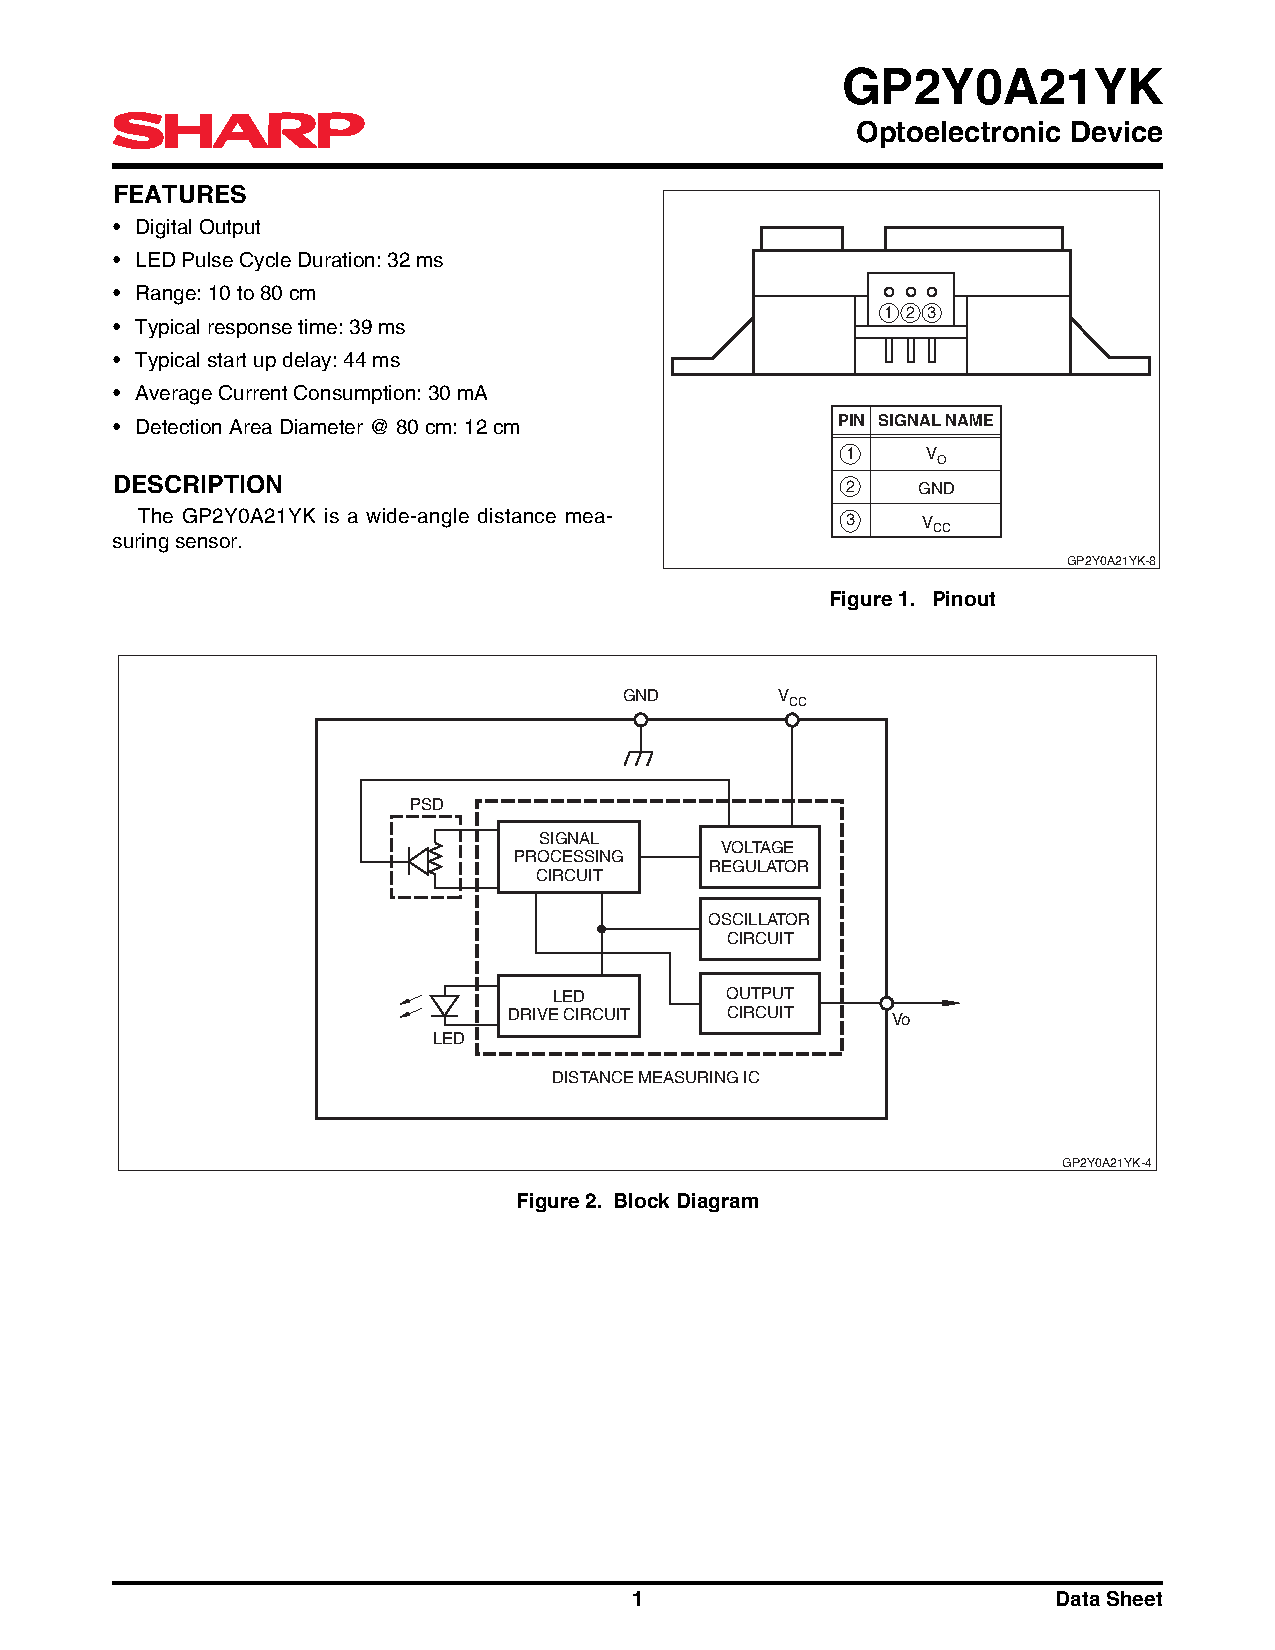
\includepdf[pages=1]{datasheets/SharpDatasheet.pdf}
%
%\cleardoublepage

%
%\chapter{Something Else}\label{sec:something}
%
%Add here some other appendix material \dots
%
% \cleardoublepage
 
 
 

